\documentclass[9pt]{beamer}
%The used theme. Options: No page number, progress bar at the bottom, no standalone frames for section titles
\usetheme[numbering=fraction,progressbar=none,sectionpage=none,block=fill,numbering=none]{metropolis}
%%This is used for smoothly blending the backgrounds of navigation and frame title
\useoutertheme[subsection=true]{smoothbars}
%This is to smoothly integrate the sections in the navigation
\setbeamercolor{section in head/foot}{fg=white,bg=mDarkTeal}
\setbeamercolor{subsection in head/foot}{fg=white,bg=mDarkTeal}
%
%
%%I don't really remember what this does. I guess it makes the header look good?
%\setbeamertemplate{headline}{%
%\begin{beamercolorbox}[colsep=1.5pt]{upper separation line head}
%\end{beamercolorbox}
%\begin{beamercolorbox}{section in head/foot}
%\insertsectionnavigationhorizontal{\paperwidth}{}{}
%\end{beamercolorbox}
%\begin{beamercolorbox}{subsection in head/foot}
%\insertsubsectionnavigationhorizontal{\paperwidth}{}{}
%\end{beamercolorbox}
%}
\setbeamertemplate{headline}{%
\begin{beamercolorbox}[colsep=1.5pt]{upper separation line head}
\end{beamercolorbox}
\begin{beamercolorbox}{section in head/foot}
    \vskip2pt\insertsectionnavigationhorizontal{\paperwidth}{}{\hskip0pt plus1filll}\vskip2pt
\end{beamercolorbox}%
\begin{beamercolorbox}[ht=10pt]{subsection in head/foot}%
    \vskip2pt\insertsubsectionnavigationhorizontal{\paperwidth}{}{\hskip0pt plus1filll}\vskip2pt
\end{beamercolorbox}%
\begin{beamercolorbox}[colsep=1.5pt]{lower separation line head}
\end{beamercolorbox}
}
%
%%Numbered definitions
%\setbeamertemplate{theorems}[numbered]
%
%%Puts the section numbers in circles in the ToC
%\setbeamertemplate{section in toc}[circle]
%We don't want frames that are broken into multiple slides to have these slides numbered
\setbeamertemplate{frametitle continuation}{}

%Changing fonts
\usepackage{fontspec}
%Not using the official Uni Bern font since there's gonna be lots of IPA. Using Calibri for true smallcaps.
%\setsansfont{Frutiger LT Com 55 Roman}
\setsansfont[SmallCapsFont=Calibri,SmallCapsFeatures={RawFeature=+smcp,Scale=1.1}]{DejaVu Sans}

%Drawing facilities
\usepackage{tikz}
\usetikzlibrary{positioning}
%For consistent quotation marks
\providecommand{\dbqu}[1]{``#1''}
\providecommand{\subs}[1]{\textsubscript{#1}}

%For formatting URLs
\usepackage{url}

%This package provides symbols
\usepackage[misc]{ifsym}
\usepackage{fontawesome}
%Author definition contains a mailto link
\author{Florian Matter \href{mailto:florian.matter@isw.unibe.ch}{\faEnvelopeO}}
\institute{Institut für Sprachwissenschaft, Universität Bern}

%For intelligent cross-references
\usepackage[noabbrev,nameinlink]{cleveref}

\usepackage{tabularx}
\usepackage{booktabs}
%Configure table rules for easier adaptation
\newcommand{\mytoprule}{\toprule}
\newcommand{\mymidrule}{\midrule}
\newcommand{\mybottomrule}{\bottomrule}

\usepackage{xspace}
\providecommand{\goodtilde}{\char`~\xspace}

%For multicolumn lists on slides
\usepackage{multicol}

\usepackage{tikz-qtree}
\usetikzlibrary{tikzmark}

%Just for emphasis
\newcommand{\emp}[1]{\textbf{#1}}

\hypersetup{
    colorlinks = true,
    linkcolor = {orange},
    urlcolor = {orange},
    citecolor = {orange},
    filecolor = {orange},
    linkbordercolor = {orange},
}

%Enables underlined and colored links
\makeatletter
\Hy@AtBeginDocument{%
  \def\@pdfborder{0 0 1}% Overrides border definition set with colorlinks=true
  \def\@pdfborderstyle{/S/U/W 1}% Overrides border style set with colorlinks=true
                                % Hyperlink border style will be underline of width 1pt
}
\makeatother
\input{glossingConfigurationBeamer}
\usepackage{datetime2}
\usepackage{phonrule}
\usepackage[edges]{forest}
\input{iswbibConfiguration}
\addbibresource{cariban_references.bib}
\usepackage{xspace}
\providecommand{\wbakairi}{Western Bakairi\xspace}
\providecommand{\ebakairi}{Eastern Bakairi\xspace}
\providecommand{\ingariko}{Ingarikó\xspace}
\providecommand{\akawaio}{Akawaio\xspace}
\providecommand{\patamona}{Patamona\xspace}
\providecommand{\yukpa}{Yukpa\xspace}
\providecommand{\japreria}{Japreria\xspace}
\providecommand{\carijo}{Karijona\xspace}
\providecommand{\mapoyo}{Mapoyo\xspace}
\providecommand{\yawarana}{Yawarana\xspace}
\providecommand{\panare}{Panare\xspace}
\providecommand{\maqui}{Ye'kwana\xspace}
\providecommand{\pemon}{Pemón\xspace}
\providecommand{\kapon}{Kapong\xspace}
\providecommand{\waimiri}{Waimiri-Atroari\xspace}
\providecommand{\macushi}{Macushi\xspace}
\providecommand{\waiwai}{Waiwai\xspace}
\providecommand{\hixka}{Hixkaryána\xspace}
\providecommand{\kaxui}{Werikyana\xspace}
\providecommand{\trio}{Tiriyó\xspace}
\providecommand{\akuriyo}{Akuriyó\xspace}
\providecommand{\apalai}{Apalaí\xspace}
\providecommand{\wayana}{Wayana\xspace}
\providecommand{\ikpeng}{Ikpeng\xspace}
\providecommand{\arara}{Arara\xspace}
\providecommand{\kalina}{Kari'ña\xspace}
\providecommand{\uxc}{Upper Xingu Carib\xspace}
\providecommand{\bakairi}{Bakairi\xspace}
\providecommand{\PC}{Proto-Cariban\xspace}
\providecommand{\PPar}{Proto-Parukotoan\xspace}
\providecommand{\PWai}{Proto-Waiwaian\xspace}
\providecommand{\PPek}{Proto-Pekodian\xspace}
\providecommand{\PXin}{Proto-Xinguan\xspace}
\providecommand{\PPP}{Proto-Pemong-Panare\xspace}
\providecommand{\PTar}{Proto-Taranoan\xspace}
\providecommand{\PTir}{Proto-Tiriyoan\xspace}

\newcommand{\pcone}{\\\small\begin{tabular}{@{}rllll@{}}
& \gl{a} & \gl{s_a_} & \gl{s_p_} & \gl{p}\\
\gl{1} & \rc{t(i)-} & \rc{w-} & \rc{u(j)-} & \rc{u(j)-}\\
\gl{2} & \rc{m(i)-} & \rc{m-} & \rc{ə(j)-} & \rc{ə(j)-}\\
\gl{1+2} & \rc{kɨt(i)-} & \rc{kɨt-} & \rc{k-} & \rc{k-}\\
\end{tabular}}

\newcommand{\ppone}{\\\small\begin{tabular}{@{}rllll@{}}
& \gl{a} & \gl{s_a_} & \gl{s_p_} & \gl{p}\\
\gl{1} & \emp{\rc{w-}} & \rc{w-} & \emp{\rc{k-}} / *Ø/\obj{j-} & *Ø/\obj{j-}\\
\gl{2} & \rc{m-} & \rc{m-} & \rc{o(j)-} & \rc{o(j)-}\\
\gl{1+2} & \rc{kɨt-} & \rc{kɨt-} & \rc{k-}, \emp{\rc{kɨt-}} & \rc{k-}\\
\end{tabular}}

\newcommand{\kaxone}{\\\small\begin{tabular}{@{}rllll@{}}
& \gl{a} & \gl{s_a_} & \gl{s_p_} & \gl{p}\\
\gl{1} & \obj{w-} & \obj{w-} & \obj{k-}, Ø/\obj{j-} & Ø/\obj{j-}\\
\gl{2} & \obj{m-} & \obj{m-} & \obj{o-} & \obj{o-}\\
\gl{1+2} & \obj{kɨt-} & \obj{kɨt-} & \obj{k-} / \obj{kɨt-} & \obj{k-}\\
\end{tabular}}

\newcommand{\pwone}{\\\small\begin{tabular}{@{}rllll@{}}
& \gl{a} & \gl{s_a_} & \gl{s_p_} & \gl{p}\\
\gl{1} & \rc{w-} & \emp{\rc{k-}} & \rc{k-} & \emp{\rc{owɨ(ro) j-}}\\
\gl{2} & \rc{m-} & \rc{m-} & \rc{o(j)-} & \rc{o(j)-}\\
\gl{1+2} & \rc{tɨt-} & \rc{tɨt-} & \rc{tɨt-} & \rc{k-}\\
\end{tabular}}

\newcommand{\hixone}{\\\small\begin{tabular}{@{}rllll@{}}
& \gl{a} & \gl{s_a_} & \gl{s_p_} & \gl{p}\\
\gl{1} & \obj{w-}/\obj{ɨ-} & \obj{k-} & \obj{k-} & \obj{r(o)-}\\
\gl{2} & \obj{m-} & \obj{m-} & \obj{o(j)-} & \obj{o(j)-}\\
\gl{1+2} & \obj{t-} & \obj{t-} & \obj{t-} & \obj{k-}\\
\end{tabular}}

\newcommand{\waione}{\\\small\begin{tabular}{@{}rllll@{}}
& \gl{a} & \gl{s_a_} & \gl{s_p_} & \gl{p}\\
\gl{1} & \obj{w-} & \obj{k-} & \obj{k-} & \obj{o(j)-}\\
\gl{2} & \obj{m-} & \obj{m-} & \emp{\obj{m-}} & \obj{a(w)-}\\
\gl{1+2} & \obj{t(ɨt)-} & \obj{t(ɨt)-} & \obj{t(ɨt)-} & \obj{k-}\\
\end{tabular}}

\newcommand{\setone}{Set I\xspace}
\addbibresource{non_cariban_references.bib}
\title{Irregular first person inflections in Cariban: converging factors for morphological (dis-)similarity}
\institute{SLE 2021 (Online)}
\date{\DTMdate{2021-08-31}}

\begin{document}

\frame{\maketitle}

\section{Irregular first person inflections}

\subsection{Cariban verbal person marking}

\begin{frame}{\PC \setone (main clause) person markers}
	\begin{tabular}{@{}lllll@{}}
	\mytoprule
\gl{a}/\gl{p}&		\gl{1}	&	\gl{2}		&	\gl{1+2}	&	\gl{3}	\\
\mymidrule
\gl{1}	&		&	\rc{k-}	&				&	\rc{t(i)-}		\\	
\gl{2}	&	\rc{k-}			&&				&	\rc{m(i)-}		\\
\gl{1+2}&		&				&				&	\rc{kɨt(i)-}		\\
\gl{3}	&	\rc{u(j)-}	&	\rc{ə(j)-}	&	\rc{k-}			&	\rc{n(i)-}		\\
	\mybottomrule
	\end{tabular}
	\hfill
\begin{tabular}{@{}lll@{}}
\mytoprule
& \gl{s_a_} & \gl{s_p_}  \\
\mymidrule
\gl{1} & \rc{w-} & \rc{u(j)-} \\
\gl{2} & \rc{m-} & \rc{ə(j)-}\\
\gl{1+2} & \rc{kɨt-} & \rc{k-}\\
\gl{3} & \rc{n-} & \rc{n(i)-}\\
\mybottomrule
\end{tabular}	
\end{frame}

\begin{frame}{The split-\gl{s} system}
\begin{itemize}
	\item conserved in many modern languages
	\item \gl{p}-markers identical to \gl{s_p_}
	\item \gl{a}-markers = \gl{s_a_} + \rc{i-} (except first person)
	\item \emp{no semantic basis} (\hyperlink{kalina}{illustration})
\end{itemize}
\end{frame}

\begin{frame}{What conditions the split? \parencite{meira2000split}}
\begin{itemize}
	\item not explicable by (non\-)activities, (non-)agency, (in-)animacy, Aktionsart
	\item purely lexical, semantically arbitrary
	\item but: vast majority of \gl{s_a_} verbs have reflex of detransitivizer \rc{ət(e)-}/\obj{e-}
	\item derivational prefix attaching mostly to transitive verbs, with various semantics (\hyperlink{triodetrz}{illustration})
\end{itemize}
\end{frame}

\subsection{Person marker extensions}
\begin{frame}{Example for person marker extensions: Parukotoan \parencite[94]{gildea1998}}
\centering
\begin{tikzpicture}[
	every node/.append style={align=center},
	level distance=100pt
]
\tikzset{edge from parent/.append style={thick,->}}
\Tree[.\node[draw]{\PC{}\pcone};
\node[draw]{\PPar{}\\\small\begin{tabular}{@{}rllll@{}}
& \gl{a} & \gl{s_a_} & \gl{s_p_} & \gl{p}\\
\gl{1} & \subnode{ppar13}{\emp{\rc{w-}}} & \subnode{ppar1w}{\rc{w-}} & \emp{\rc{k-}} / *Ø/\obj{j-} & *Ø/\obj{j-}\\
\gl{2} & \rc{m-} & \rc{m-} & \rc{o(j)-} & \rc{o(j)-}\\
\gl{1+2} & \rc{kɨt-} & \rc{kɨt-} & \rc{k-}, \emp{\rc{kɨt-}} & \rc{k-}\\
\end{tabular}};
%{\kaxui{}\kaxone}
%[.{\PWai{}\pwone}
%{\hixka{}\hixone}
%{\waiwai{}\waione}
%]
%]
]
\end{tikzpicture}
% \begin{tikzpicture}[overlay,>=latex,shorten >=1pt,->,remember picture]
% \draw[black, ->] (ppar1w) -- (ppar13);
%\end{tikzpicture}
\end{frame}

\begin{frame}{Example for person marker extensions: Parukotoan}
\centering
\begin{tikzpicture}[
	every node/.append style={align=center,scale=0.9},
	level distance=100pt,
]
\tikzset{edge from parent/.append style={thick,->}}
\Tree[.\node[draw]{\PPar\\\small\begin{tabular}{@{}rllll@{}}
& \gl{a} & \gl{s_a_} & \gl{s_p_} & \gl{p}\\
\gl{1} & \rc{w-} & \rc{w-} & \rc{k-} / *Ø/\obj{j-} & *Ø/\obj{j-}\\
\gl{2} & \rc{m-} & \rc{m-} & \rc{o(j)-} & \rc{o(j)-}\\
\gl{1+2} & \rc{kɨt-} & \rc{kɨt-} & \rc{k-}, \rc{kɨt-} & \rc{k-}\\
\end{tabular}};%{\PPar{}}
\node[draw]{\kaxui{}\kaxone};
\node[draw]{\PWai{}\pwone};
%{\hixka{}\hixone}
%{\waiwai{}\waione}
%]
%]
]
\end{tikzpicture}
\end{frame}

\begin{frame}{Example for person marker extensions: Parukotoan}
\centering
\begin{tikzpicture}[
	every node/.append style={align=center},
	level distance=100pt,
]
\tikzset{edge from parent/.append style={thick,->}}
\Tree[.\node[draw,label=above:\PWai{}]{\small\begin{tabular}{@{}rllll@{}}
& \gl{a} & \gl{s_a_} & \gl{s_p_} & \gl{p}\\
\gl{1} & \rc{w-} & \rc{k-} & \rc{k-} & \rc{owɨ(ro) j-}\\
\gl{2} & \rc{m-} & \rc{m-} & \rc{o(j)-} & \rc{o(j)-}\\
\gl{1+2} & \rc{tɨt-} & \rc{tɨt-} & \rc{tɨt-} & \rc{k-}\\
\end{tabular}};
\node[draw]{\hixka{}\hixone};
\node[draw]{\waiwai{}\waione};
%]
%]
]
\end{tikzpicture}
\end{frame}

\begin{frame}{Person marker extensions: lexical diffusion}
\begin{itemize}
	\item gradual spread through the verbal lexicon, not all at once: \begin{enumerate}
	\item visible in ongoing changes in \kaxui
	\item place switch of \PC \rc{t-} (\gl{1}>\gl{3}) and \rc{w-} (\gl{1}\gl{s_a_}) in Tiriyoan likely by lexical diffusion \parencite[112]{meira1998proto}
	\item incomplete extensions -- diffusion stops short of some verbs
\end{enumerate}
\end{itemize}
\end{frame}

\subsection{Incomplete extensions}
%\begin{frame}{Incomplete extensions}
%\begin{itemize}
%	\item t \exref{arasa}
%\end{itemize}
%\ex<arasa> \arara \gl{s_a_} verbs\\ \parencite[61, 99, 150, 164, 177]{alves2017arara} \\
%\begin{tabular}[t]{@{}llll@{}}
%&  \qu{to dance} & \qu{to enter} & \qu{to bathe}\\
%\gl{1} & \obj{k-origu-} & \obj{k-omomɨ-} & \obj{\emp{w-}ibɨ-}\\
%\gl{2} & \obj{m-origu-} & \obj{m-omomɨ-} & \obj{m-ibɨ-}\\
%\gl{1+2} & \obj{kud-origu-} & \obj{kut-omomɨ} & \obj{kut͡ʃ-ibɨ-}\\
%\gl{3} & Ø-\obj{origu} & Ø-\obj{omomɨ-} & Ø\obj{-ibɨ-}\\
%\end{tabular}
%\xe
%\end{frame}

\begin{frame}{Incomplete extension: \PPek \rc{k-}}
\label{ppek}
%\begin{itemize}
%	\item likely from \gl{1+2}\gl{s_p_} prefix \rc{k-}
%%	\item so far no reconstructions of \PPek
%	\item newly identified shared innovation of the Pekodian branch
%\end{itemize}
\ex<pekreg>
\begin{tabular}[t]{@{}llll@{}}
 & \arara \qu{to dance}  & \ikpeng \qu{to run} & \bakairi \qu{to go up} \\
& \parencite[150]{alves2017arara} &  \parencite[52]{ikpengpacheco2001}& \parencite[4]{meira2003bakairi} \\
\gl{1}\gl{s_a_}  & \obj{\emp{k-}origu-} & \obj{\emp{k-}aranme-} & \obj{\emp{k-}əku-}\\
\gl{2}\gl{s_a_}  & \obj{m-origu-} & \obj{m-aranme-} & \obj{m-əku-}\\
\gl{1+2}\gl{s_a_}  & \obj{kud-origu-} & \obj{kw-aranme-} & \obj{kɨd-əku-}\\
\gl{3}\gl{s_a_} & \obj{Ø-origu-} & \obj{Ø-aranme-} & \obj{n-əku-}\\
\end{tabular}
\xe
\end{frame}

\begin{frame}{\PPek \rc{k-}: unaffected verbs}
\begin{itemize}
	\item those verbs not affected by specific extension retain old markers -- \dbqu{irregular} or \dbqu{archaic}
\end{itemize}
\begin{center}
\begin{tabular}{@{}lllll@{}}
	\mytoprule
& \PPek & \arara & \ikpeng & \bakairi \\
\mytoprule
\qu{say} & \rc{wɨ-ge-} & \obj{wɨ-ge-} & \obj{ɨ-ge-} & \obj{u-ge-} \\
\qu{bathe} & \rc{w-ipɨ-} & \obj{w-ibɨ-} & \obj{Ø-ip-} & \obj{w-i-} \\
\qu{be} & \rc{w-et͡ʃi-} & \obj{w-it͡ʃi-} & \obj{Ø-et͡ʃi-} & \obj{w-i-} \\
& \rc{w-ap-} & \obj{w-ap-} & -- & \obj{w-a-}\\
\qu{come} & \rc{w-epɨ} / \rc{k-əd-epɨ-} & \obj{w-ebɨ-} & \obj{k-arep-} & \obj{k-əewɨ-} \\
\qu{go down} & \rc{w-[ɨ/i]ptə-} & \obj{w-iptoŋ-} & ?\obj{-iptoŋ-} & \obj{k-ɨtəgɨ-} \\
\qu{go} & \rc{w-ɨtən-} & \obj{w-ɨdo-} & \obj{k-aran-} & \obj{u-tə-} \\
	\mybottomrule
	\end{tabular}\\
\footnotesize \parencites[153, 200]{alves2017arara}[130]{von1892bakairi}[4]{meira2003bakairi}[80, 139, 209]{ikpengpacheco2001}[68; p.c., Angela Fabíola Alves Chagas]{ikpengpacheco1997}
\end{center}
\end{frame}

\begin{frame}{\qu{to come} in Pekodian}
\small
\begin{itemize}
	\item \ikpeng \obj{k-arep-} and \bakairi \obj{k-əewɨ-} point to \rc{k-əd-ebɨ} (root \rc{ebɨ} with detransitivizing prefix)
	\item \arara \obj{w-ebɨ-} points to \rc{w-ebɨ-} (bare root)
	\item \arara also has reflexes of complex \rc{əd-ebɨ} elsewhere in the paradigm \exref{ara-123}
	\item extension of \rc{k-} to morphologically complex form either in \PPek (coexisting variants), or subsequently in daughters (paradigm leveling)
\end{itemize}
\ex<ara-123> \arara \parencite[][150]{alves2017arara}
\begingl
\gla m-odebɨ-nɨ//
\glb \gl{2}\gl{s_a_}-come-\gl{rec}//
\glft \qu{You came.}//
\endgl
\xe

\end{frame}

\begin{frame}{Incomplete person marker extensions in Cariban}
\begin{itemize}
	\item six incomplete extensions (of 19 investigated extensions)
	\item \emp{all innovative \gl{1}\gl{s_a_} markers}
	\item i.e., what remains is a small class of verbs with reflexes of \PC \gl{1}\gl{s_a_} \rc{w-}
	\item other extensions: \begin{itemize}
	\item non-first persons only innovate \gl{s_p_} markers, never \gl{s_a_}
	\item always affect all verbs (unless still ongoing)\end{itemize}
\end{itemize}
\end{frame}

\begin{frame}{Incomplete extensions of new \gl{1}\gl{s_a_} markers}
\begin{enumerate}
	\item \PPek \rc{k-} (\hyperlink{sec:ppek}{details})
	\item \PWai \rc{k-} (\hyperlink{sec:pwai}{details})
	\item \PTir \rc{t-} (\hyperlink{sec:ptir}{details})
	\item \akuriyo \obj{k-} (\hyperlink{sec:aku}{details})
	\item \carijo \obj{j-} (\hyperlink{sec:car}{details})
	\item \yukpa \obj{j-} (\hyperlink{sec:yuk}{details})
\end{enumerate}
\end{frame}

\begin{frame}{Distribution in the family}
\begin{figure}
\centering
\tiny
\begin{forest}
for tree={
s sep = -1ex,
grow=east,
forked edges,
node options={align=center },
anchor=west,edge path={\noexpand\path[draw, gray, line width=1pt, \forestoption{edge}](!u.parent anchor) |- (.child anchor)\forestoption{edge label};},
before typesetting nodes={if content={}{shape=coordinate}{}},}
    [Cariban, tier=4
        [
            [{\uxc}, tier=0]
        ]
        [
            [{\waimiri}, tier=0]
        ]
        [
            [{\apalai}, tier=0]
        ]
        [
            [{\wayana}, tier=0]
        ]
        [
            [{\kalina}, tier=0]
        ]
        [Yukpan,tier=1
            [{\emp{\yukpa}}, tier=0]
            [{\japreria}, tier=0]
        ]
        [Taranoan, tier=2
            [\emp{Tiriyoan}
                [{\trio}, tier=0]
                [{\emp{\akuriyo}}, tier=0]
            ]
            [{\emp{\carijo}}, tier=0]
        ]
        [Venezuelan, tier=3
            [{\maqui/\dekwana}, tier=0]
            [Core Venezuelan, tier=2
            	[%\pemon-\panare
            	[{\panare}, tier=0]
                [Pemongan, tier=1
                    [{\ingariko}, tier=0]
                    [{\macushi}, tier=0]
                    [{\pemon}, tier=0]
                ]
            	]
            	[
            	  [{\kumana}, tier=0]
                [{\tamanaku}, tier=0]
                [
                [{\mapoyo}, tier=0]
                [{\yawarana}, tier=0]
                ]
            	]
            ]
        ]
        [\emp{Pekodian}, tier=2
            [Xinguan, tier=1
                [{\arara}, tier=0]
                [{\ikpeng}, tier=0]
            ]
            [{\bakairi}, tier=0]
        ]
        [Parukotoan, tier=2
            [\emp{Waiwaian}, tier=1
                [{\hixka}, tier=0]
                [{\waiwai}, tier=0]
            ]
            [{\kaxui}, tier=0]
        ]
    ]
\end{forest}
\caption{The Cariban language family}
\label{fig:caribantree}
\end{figure}
\end{frame}

\begin{frame}{Geographical distribution}
\begin{center}
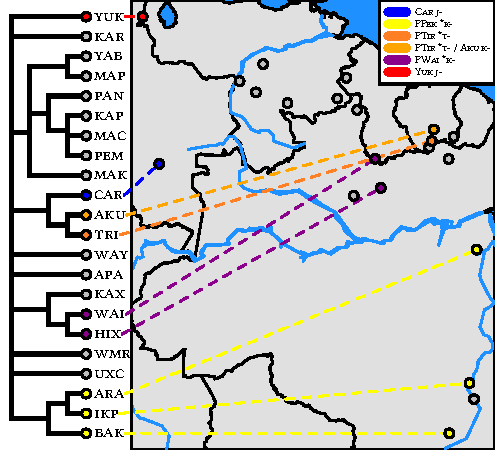
\includegraphics[height=0.9\textheight]{stuff/cariban_phylo_map}
\end{center}
\end{frame}



%\begin{frame}{Example: regular \gl{s_a_} in Pekodian}
%\footnotesize
%\begin{tabular}[t]{@{}llll@{}}
%\mytoprule
%& \bakairi \qu{to go up}  & \arara \qu{to dance}  & \ikpeng \qu{to run} \\
%& \parencite[4]{meira2003bakairi} & \parencite[150]{alves2017arara} &  \parencite[52]{ikpengpacheco2001}\\
%\mymidrule
%\gl{1}\gl{s_a_} & \obj{\emp{k-}əku-} & \obj{\emp{k-}origu-} & \obj{\emp{k-}aranme-} \\
%\gl{2}\gl{s_a_} & \obj{m-əku-} & \obj{m-origu-} & \obj{m-aranme-} \\
%\gl{1+2}\gl{s_a_} & \obj{kɨd-əku-} & \obj{kud-origu-} & \obj{kw-aranme-} \\
%\gl{3}\gl{s_a_} & \obj{n-əku-} & \obj{Ø-origu-} & \obj{Ø-aranme-} \\
%\mybottomrule
%\end{tabular}
%\end{frame}
%
%\begin{frame}{Example: irregular \gl{1}\gl{s_a_} in Pekodian}
%\footnotesize
%	\begin{tabular}{@{}lllll@{}}
%	\mytoprule
%& \PPek & \arara & \ikpeng & \bakairi \\
%\mytoprule
%\qu{say} & \rc{wɨ-ge-} & \obj{wɨ-ge-} & \obj{ɨ-ge-} & \obj{u-ge-} \\
%\qu{bathe} & \rc{w-ipɨ-} & \obj{w-ibɨ-} & \obj{Ø-ip-} & \obj{w-i-} \\
%\qu{be} & \rc{w-et͡ʃi-} & \obj{w-it͡ʃi-} & \obj{Ø-et͡ʃi-} & \obj{w-i-} \\
%\qu{come} & \rc{w-epɨ}, \rc{k-əd-epɨ-} & \obj{w-ebɨ-} & \obj{k-arep-} & \obj{k-əewɨ-} \\
%\qu{go} & \rc{w-ɨtən-} & \obj{w-ɨdo-} & \obj{k-aran-} & \obj{u-tə-} \\
%\qu{go down} & \rc{w-[ɨ/i]ptə-} & \obj{w-iptoŋ-} & ?\obj{-iptoŋ-} & \obj{k-ɨtəgɨ-} \\
%	\mybottomrule
%	\end{tabular}
%\end{frame}

\begin{frame}{What verbs are unaffected by extensions?}
\small
\begin{center}
	\begin{tabular}{@{}lllllll@{}}
	\mytoprule
PC & \PPeks \rc{k-} & \PWais \rc{k-} & \PTirs \rc{t-} & \acs{aku_lg} \obj{k-} & \acs{car_lg} \obj{j-} & \acs{yuk_lg} \obj{j-} \\
\mymidrule
\rc{ɨtə(mɨ)} \qu{go} & × & × & × & × & × & × \\
\rc{ka(ti)} \qu{say} & × & × & × & × & ? & ? \\
\rc{(ət-)jəpɨ} \qu{come} & \checkmark/× & -- & × & × & \checkmark & -- \\
%\rc{ət-epɨ} \qu{come} & \checkmark & -- & × & -- & -- & -- \\
%\rc{jəpɨ} \qu{come} & × & -- & × & × & \checkmark & -- \\
\rc{ɨpɨtə} \qu{go down} & × & -- & × & × & \checkmark & -- \\
\rc{eti} \qu{be} & × & × & × & × & \checkmark & \checkmark \\
\rc{a(p)} \qu{be} & × & × & × & × & × & \checkmark \\
\rc{e-pɨ} \qu{bathe} & × & \checkmark & \checkmark & × & ? & -- \\
	\mybottomrule
	\end{tabular}\\
\emp{\checkmark} innovative marker \quad \emp{×} archaic marker\quad \emp{--} unattested \quad\emp{?} unknown
\end{center}
\begin{itemize}
	\item strong overlap among languages in the verbs retaining \gl{1}\gl{s_a_} \rc{w-}
	\item not shown: 1) many \obj{e}-initial \akuriyo verbs, 2) 4 \akuriyo movement verbs, 3) \trio \qu{to defecate}
\end{itemize}
\end{frame}

\subsection{Potential causes}
\begin{frame}{What causes verbs to adapt or resist innovative markers?}
%\small
\begin{itemize}
	\item possible explanations based on the network model of morphology by \textcites{bybee1985morphology}{bybee1995regular}:
\begin{enumerate}
	\item morphology-based lexical connections → same inflection class
	\item phonology-based lexical connections → same inflection class
	\item frequency: high-frequency lexemes are resistant to innovation
	\item (semantics play no role in this case)
\end{enumerate}
	\item strong overlap of all three factors in the Cariban case:\begin{enumerate}
	\item vast majority of \gl{s_a_} verbs have reflex of detransitivizer \rc{ət(e)-}/\obj{e-}
	\item therefore, they are \obj{e}- or \obj{ə}/\obj{o}-initial
	\item other, underived \gl{s_a_} verbs often high-frequency
	\end{enumerate}
\end{itemize}
\end{frame}

\begin{frame}{Morphology: \PPek}
\begin{itemize}
	\item none of the unaffected verbs have detransitivizer
	\item normally detransitivized \rc{e-pɨ} \qu{to bathe} has become \rc{ibɨ} in \PPek (\hyperlink{tobathe}{details})\begin{itemize}
	\item[→] loss of transparent morphology, not affected by innovative marker \end{itemize}
	\item \bakairi and \ikpeng show \rc{k-} with \rc{əd-ebɨ} \qu{to come}, but \arara has \rc{w-} with root \rc{ebɨ} (\hyperlink{tocome}{details})\begin{itemize}
	\item[→] presence of detransitivizer clearly triggers innovative prefix\end{itemize}
\end{itemize}
\end{frame}

\begin{frame}[allowframebreaks]{Phonology: \akuriyo, \carijo, \yukpa}
\begin{itemize}
	\item \akuriyo \obj{k-} only on \obj{ə}-initial verbs, not \obj{e}-initial (\hyperlink{aku}{details})
	\item \carijo: all \obj{e}- and \obj{ə}-initial verbs affected, even those without detransitivizer \exref{care}
	\item \yukpa: all V-initial verbs, only \obj{to} \qu{to go} unaffected (\hyperlink{yukpaj}{details}) -- but very patchy data!
\end{itemize}
\footnotesize
\pex<care>\carijo
\a<car-18>
\begingl
\gla əji-wa-e \emp{j-e}h-ɨ//
\glb \gl{2}-search-\gl{sup} \gl{1}-come-\gl{pfv}//
\glft \qu{I came looking for you.} \parencite[][102]{guerrero2019carijo}//
\endgl
\a<car-32>
\begingl
\gla irə wat͡ʃinakano tae \emp{j-e}hɨtə-e//
\glb \gl{inan}.\gl{ana} body.of.water along.bounded \gl{1}-go.down-\gl{npst}//
\glft \qu{…I go down through that guachinacán.} (p.c., David Felipe Guerrero)//
\endgl
\a<mivida-12>
\begingl
\glpreamble iretibə et͡ʃinəme gərə jet͡ʃiɨ//
\gla ireti-bə et͡ʃi-nə=me gərə \emp{j-e}t͡ʃi-ɨ//
\glb then-from be-\gl{inf}=\gl{attrz} still \gl{1}-be-\gl{pfv}//
\glft \qu{Then I was already grown up.} \parencite[][177]{robayo1989rame}//
\endgl
\xe
\end{frame}

\begin{frame}{Converging factors}
\begin{itemize}
	\item most resistant verbs: \rc{ka(ti)} \qu{to say} and \rc{ɨtə(mɨ)} \qu{to go}\begin{enumerate}
	\item no detransitivizer
	\item C-initial (in these languages)
	\item very frequent (although no text counts)
	\end{enumerate}
\item often no definite answer for resistance to innovation
\item \PC: underived \gl{s_a_} verbs also most frequent, other irregularities
\item ultimate origins of split-\gl{s} system still mysterious
\end{itemize}
\end{frame}

\renewcommand*{\bibfont}{\tiny}
\begin{frame}[allowframebreaks]{References}
\printbibliography
\end{frame}

\section{appx: Individual extensions}

\subsection{\PPek \rc{k-}}
\label{sec:ppek}
\begin{frame}{Irregular \arara verbs}
\ex<arairr> \arara \parencite[153]{alves2017arara} \\
\begin{tabular}[t]{@{}ll@{}}
\obj{wɨ-ge-nɨ} & \qu{I said}\\
\obj{w-it͡ʃi-nɨ} & \qu{I was, lied down}\\
\obj{w-ebɨ-nɨ} & \qu{I came}\\
\obj{w-ibɨ-nɨ} & \qu{I bathed}\\
\obj{w-iptoŋ-rɨ} & \qu{I went down}\\
\obj{w-ɨdo-lɨ} & \qu{I went}\\
\end{tabular}
\xe
\end{frame}

\begin{frame}{Cognate verbs in \bakairi: \obj{u-}/\obj{w-}, two \obj{k-}}
\footnotesize
\pex[everyglpreamble=,interpartskip=-1ex]<bakverbs> \bakairi \parencites[][131, 397, 76, 137, 374]{von1892bakairi}[4]{meira2003bakairi}
\begin{multicols}{2}
\a<bak-3>
\begingl
\glpreamble \ort{u-ɣépa} //
\gla \emp{u-}ge-pa//
\glb \gl{1}\gl{s_a_}-say-\gl{neg}//
\glft \qu{I don't say.}//
\endgl
\a<bak-5>
\begingl
\glpreamble \ort{wi-táki} / \ort{wi-tági} //
\gla \emp{w-}i-taki//
\glb \gl{1}\gl{s_a_}-be-\gl{int}//
\glft \qu{I was.}//
\endgl
\a<bak-4>
\begingl
\glpreamble \ort{kχaewí-le} //
\gla \emp{k-}əewɨ-lɨ//
\glb \gl{1}\gl{s_a_}-come-\gl{imm}//
\glft \qu{I came.}//
\endgl
\a<bak-6>
\begingl
\glpreamble \ort{kχ-itaké-he} //
\gla \emp{k-}ɨtəgɨ-se//
\glb \gl{1}\gl{s_a_}-go.down-\gl{npst}?//
\glft \qu{I go down.}//
\endgl
\a<bak-2>
\begingl
\glpreamble \ort{ū́ta} / \ort{uúta}//
\gla \emp{u-}tə//
\glb \gl{1}\gl{s_a_}-go//
\glft \qu{I go.}//
\endgl
\a
\begingl
\gla \emp{w-}i-də//
\glb \gl{1}\gl{s_a_}-bathe-\gl{imm}//
\glft \qu{I bathed}//
\endgl
\end{multicols}
\xe
\end{frame}

\begin{frame}[allowframebreaks]{Cognate verbs in \ikpeng: \obj{ɨ-}/Ø-, two \obj{k-}}
\small
\pex<ikpw>
\a<ikp-168>
\begingl
\gla \emp{ɨ-}ge-lɨ//
\glb \gl{1}-say-\gl{rec}//
\glft \qu{I said.} \parencite[][209]{ikpengpacheco2001}//
\endgl
\a<ikp-169>
\begingl
\gla \emp{Ø-}et͡ʃi-lɨ//
\glb \gl{1}-be-\gl{rec}//
\glft \qu{I was.} \parencite[][139]{ikpengpacheco2001}//
\endgl
\a<ikp-167>
\begingl
\gla at͡ʃagotpop \emp{Ø-}ip-t͡ʃi ik-gwa-kt͡ʃi//
\glb always \gl{1}-bathe-\gl{npst} river-\gl{loc}.aquatic-\gl{all}//
\glft \qu{I always bathe in this river.} \parencite[][68]{ikpengpacheco1997}//
\endgl
\xe

\pex<ikpk> Subsequent innovations:
\a<ikp-170>
\begingl
\gla \emp{k-}aran-t͡ʃi//
\glb \gl{1}-go-\gl{npst}//
\glft \qu{I'm going.} \parencite[][80]{ikpengpacheco2001}//
\endgl
\a<ikp-171>
\begingl
\gla \emp{k-}arep-lɨ//
\glb \gl{1}-come-\gl{rec}//
\glft \qu{I came.} \parencite[][80]{ikpengpacheco2001}//
\endgl
\xe
Unattested first person form: \obj{iptoŋ} \qu{to sit down} (p.c., Angela Fabíola Alves Chagas)
\end{frame}

\begin{frame}{\PPek \rc{k-}: unaffected verbs}
\begin{center}
\hyperlink{ppek}{Overview table}	
\end{center}
\end{frame}

\subsection{\PWai \rc{k-}}
\label{sec:pwai}
\begin{frame}[allowframebreaks]{\PWai \rc{k-}}
\begin{itemize}
	\item first extension of \gl{1+2}\gl{s_p_} \rc{k-} to \gl{1}\gl{s_p_} in \PPar
	\item then further extension from \gl{1}\gl{s_p_} to \gl{1}\gl{s_a_}, creating unified first person category:
\end{itemize}
\small
\ex<wais> \PWai \\
\begin{tabular}[t]{@{}lll@{}}
\gl{1} & \rc{\emp{k-}eɸurka-} & \rc{kɨ-wɨnɨkɨ-}\\
\gl{2} & \rc{m-eɸurka-} & \rc{o-wɨnɨkɨ-}\\
\gl{1+2} & \rc{t-eɸurka-} & \rc{tɨt-wɨnɨkɨ-}\\
\gl{3} & \rc{ɲ-eɸurka-} & \rc{nɨ-wɨnɨkɨ-}\\
& \qu{to fall} (\gl{s_a_}) & \qu{to sleep} (\gl{s_p_})\\
\end{tabular}
\xe
\pex Modern reflexes\\
\a \hixka \parencites[510]{howard2001wrought}[189--191]{hixkaryanaderby1985} \\ \begin{tabular}[t]{@{}lll@{}}
	\gl{1} & \obj{k-ehurka-} & \obj{kɨ-nɨkɨ-}\\
\gl{2} & \obj{m-ehurka-} & \obj{o-wnɨkɨ-}\\
\gl{1+2} & \obj{t-ehurka-} & \obj{tɨ-nɨkɨ-}\\
\gl{3} & \obj{ɲ-ehurka-} & \obj{nɨ-nɨkɨ-}\\
\end{tabular}
\a \waiwai \parencites[510]{howard2001wrought}[209--211]{hawkins1953waiwai}[50]{waiwaihawkins1998} \\ \begin{tabular}[t]{@{}lll@{}}
\gl{1} & \obj{k-eɸɨrka-} & \obj{kɨ-wɨnk-}\\
\gl{2} & \obj{m-eɸɨrka-} & \obj{mɨ-wɨnk-}\\
\gl{1+2} & \obj{t͡ʃ-eɸɨrka-} & \obj{tɨt-wɨnk-}\\
\gl{3} & \obj{ɲ-eɸɨrka-} & \obj{nɨ-wɨnk-}\\
\end{tabular}
\xe
\end{frame}

\begin{frame}{\PWai \rc{k-}: unaffected verbs}
\ex<parpar> Archaic \gl{1}\gl{s_a_} forms \\ (\cite[124, 197--198, 209]{hixkaryanaderby1985} and Spike Gildea, p.c.)\\
\begin{tabular}[t]{@{}llll@{}}
 & \PPar & \hixka & \waiwai \\
\qu{to say} & \rc{\emp{wɨ-}ka-} & \obj{\emp{ɨ-}to-} & \obj{\emp{wɨɨ-}ka}\\
\qu{to be} & \rc{\emp{w-}eʃi-}/\obj{\emp{w-}ah-} & \obj{\emp{w-}eʃe-}/\obj{\emp{w-}ah-} & \obj{\emp{w-}eeʃi-}/\obj{\emp{w-}a-}\\
\qu{to go} & \rc{\emp{wɨ-}to-} & \obj{\emp{ɨ-}to-} & \obj{kɨ\emp{w-}to-}\\
\end{tabular}\\
\xe
\end{frame}

\subsection{\PTir \rc{t-}}
\label{sec:ptir}
\begin{frame}[allowframebreaks]{\PTir \rc{t-}}
\begin{itemize}
	\item in \trio and \akuriyo, \PC \rc{t-} (\gl{1}>\gl{3}) and \rc{w-} (\gl{1}\gl{s_a_}) switched places \parencite[107--112]{meira1998proto}
	\item \envr{\rc{t-}}{\rc{ə}}, \envr{\rc{t͡ʃ-}}{\rc{e}}
	\item maybe in \PTar, maybe in \PTir{} -- \carijo removed any evidence by the \hyperlink{sec:car}{extension of \obj{j(i)-}}
\end{itemize}
\end{frame}
\begin{frame}[allowframebreaks]{\PTir \rc{t-}: unaffected verbs}
\small
\pex<ptirw> \PTir \gl{1}\gl{s_a_} \rc{w-}\\
\begin{tabular}[t]{@{}llll@{}}
& \PTir & \trio & \akuriyo\\
\qu{go} & \rc{wɨ-tə(mɨ)-} & \obj{wɨ-tə(mɨ)-} & \obj{ə-təmɨ-}/\obj{wɨ-təemɨ-}  \\
\qu{say} & \rc{wɨ-ka-} & \obj{wɨ-ka-} & \obj{wɨ-ka-} \\
\qu{come} & \rc{w-əʔepɨ-} & \obj{w-əepɨ-} & \obj{Ø-eepɨ-} \\
\qu{be} & \rc{w-ae-} & \obj{w-ae-} & Ø\obj{-aʔe-} \\
& \rc{w-eʔi-} & \obj{w-ei-} & --\\
\end{tabular}\\
\parencites[112--115]{meira1998proto}[85]{gildea1994akuriyo}[339]{triomeira1999}
\xe
\pex<akumov>
\a<aku> \akuriyo \gl{1}\gl{s_a_} \rc{w-} in 4 movement verbs\\ \parencite[84--86]{gildea1994akuriyo}\\
\begin{tabular}[t]{@{}ll@{}}
\qu{return} & Ø\obj{-erama-}\\
\qu{get up} & Ø\obj{-eokahtə-}\\
\qu{jump} & \obj{w-ejahka-}\\
\qu{go out} & \obj{w-ekɨrɨka-}\\
\end{tabular}
\a<tri> \trio \obj{s-erama-} \parencite[301]{triomeira1999}
\xe
\ex<downshit> Idiosyncratic \gl{1}\gl{s_a_} prefixes\\
\begin{tabular}[t]{@{}lll@{}}
& \trio & \akuriyo\\
\qu{go down} & \obj{p-ɨhtə-} & \obj{p-ɨtə-}\\
\qu{defecate} & \obj{k-oeka-} & ?\\
\end{tabular}\\
\parencites[294]{triomeira1999}[84]{gildea1994akuriyo}
\xe
\end{frame}

\subsection{\akuriyo \obj{k-}}
\label{sec:aku}
\begin{frame}[allowframebreaks]{\akuriyo \obj{k-}}
\label{aku}
\begin{itemize}
	\item after split of Tiriyoan, \akuriyo innovated \gl{1}\gl{s_a_} \obj{k-}
	\item apparently only replaced \rc{t-} (\envr{}{\rc{ə}}):
\end{itemize}
\begin{center}
\begin{tabular}{@{}lll@{}}
	\mytoprule
first person \obj{k-} & first person \obj{t͡ʃ-} \\
\mymidrule
\obj{ənɨkɨ} \qu{to sleep} & \obj{eepɨ} \qu{to bathe} \\
\obj{əməmɨ} \qu{to enter} & \obj{ewai} \qu{to sit down} \\
\obj{əturu} \qu{to talk} & \obj{etonema} \qu{to lie down} \\
\obj{əət͡ʃena} \qu{to cry} & \obj{ekɨɨrɨka} \qu{to stay back} \\
\obj{ətajiŋka} \qu{to run} & \obj{entapo} \qu{to yawn} \\
\obj{əiwa} \qu{to tremble} &  \\
\obj{əempa} \qu{to learn} & \parencite{gildea1994akuriyo}	\\
	\mybottomrule
	\end{tabular}
\end{center}
\begin{itemize}
	\item \textcite[107]{meira1998proto} largely agrees, mentioning \dbqu{several cases of first person \obj{t-} in \akuriyo{}} (on \obj{ə}-initial verbs)
	\item no data provided; either leftovers not affected by extension of \obj{k-}, or later influence by \trio
\end{itemize}
\end{frame}

\subsection{\carijo \obj{j-}}
\label{sec:aku}
\begin{frame}{\carijo \obj{j-}}
\begin{itemize}
	\item \carijo extended \gl{1}\gl{s_p_} \obj{j(i)-} to \gl{s_a_} verbs
	\item (alongside \gl{2}\gl{s_a_} \obj{m-} and \gl{1+2}\gl{s_a_} \obj{kɨs-} to \gl{s_p_})
\end{itemize}
\ex<carpar> \carijo \parencites[106]{meira1998proto}[173]{robayo2000avance}\\
\begin{tabular}[t]{@{}lll@{}}
& \obj{tuda} \qu{to arrive} & \obj{eharaga} \qu{to dance}\\
\gl{1} & \obj{ji-tuda-} & \obj{\emp{j-}eharaga-}\\
\gl{2} & \obj{mɨ-tuda-} & \obj{m-eharaga-}\\
\gl{1+2} & \obj{kɨsi-tuda-} & \obj{kɨs-eharaga-}\\
\gl{3} & \obj{ni-tuda-} & \obj{n-eharaga-}\\
\end{tabular}
\xe
\end{frame}
\begin{frame}{\carijo \obj{j-}: unaffected verbs}
\begin{itemize}
	\item attested are only \obj{tə} \qu{to go} and \obj{a} \qu{to be}
\end{itemize}
\pex<car1w>\carijo \parencite[][5, 42]{guerrero2016karihona}
\a<car-24>
\begingl
\gla \emp{wɨ-}tə-e=rehe//
\glb \gl{1}-go-\gl{npst}=\gl{frust}//
\glft \qu{I almost go (but I am not going to go).}//
\endgl
\a<car-25>
\begingl
\gla əji-marə-ne \emp{w-}a-e//
\glb \gl{2}-with-\gl{pl} \gl{1}-be-\gl{npst}//
\glft \qu{I am with you all.}//
\endgl
\xe
\end{frame}

\subsection{\yukpa \obj{j-}}
\label{sec:yuk}
\begin{frame}[allowframebreaks]{\yukpa \obj{j-}}
\label{yukpaj}
\begin{itemize}
	\item same innovation as \carijo{}: \gl{1}\gl{s_p_} \obj{j-} to \gl{1}\gl{s_a_} \exref{yukpaintr}
	\item not affected: only \obj{to} \qu{to go} attested \exref{yuk-7}
	\item \PC \rc{w-} is reflected as Ø \exref{yukpatr}
\end{itemize}
\ex<yukpaintr> \yukpa \parencites[72, 76]{largo2011yukpa}[139]{meira2006syntactic}\\
\begin{tabular}[t]{@{}llll@{}}
& \obj{otum} \qu{to wash self} & \obj{nɨ} \qu{to sleep} & \obj{ata} \qu{to fall}\\
\gl{1} & \obj{\emp{j-}otum-} & \obj{jɨ-nɨ-} & \obj{j-ata-}\\
\gl{2} & \obj{m-otum-} & \obj{mɨ-nɨ-} & \obj{m-ata-}\\
\gl{3} & \obj{n-otum-} & \obj{nɨ-nɨ-} & \obj{n-ata-}\\
\end{tabular}
\xe
\ex<yuk-7>\yukpa \parencite[][139]{meira2006syntactic}
\begingl
\gla aw \emp{Ø-}to//
\glb \gl{1}\gl{pro} \gl{1}\gl{s_a_}-go//
\glft \qu{I went.}//
\endgl
\xe
\pex<yukpatr>\yukpa \parencite[][139]{meira2006syntactic}
\a<yuk-5>
\begingl
\gla aw \emp{j-}esare//
\glb \gl{1}\gl{pro} \gl{3}>\gl{1}-see//
\glft \qu{S/he saw me.}//
\endgl
\a<yuk-1>
\begingl
\gla aw \emp{Ø-}esare//
\glb \gl{1}\gl{pro} \gl{1}>\gl{3}-see//
\glft \qu{I saw it.}//
\endgl
\xe
\end{frame}

\section{appx: Resistant verbs}

\subsection{\rc{ɨtə(mɨ)}}
\begin{frame}{\rc{ɨtə(mɨ)} \qu{to go}}
\label{togo}
\begin{columns}
\begin{column}{0.5\textwidth}
\begin{tabular}[t]{@{}ll@{}}
\toprule
 Language &          First person form \\
\midrule
  \waiwai &              \obj{kɨw-to-} \\
   \hixka &                \obj{ɨ-to-} \\
   \arara &               \obj{w-ɨdo-} \\
  \ikpeng &              \obj{k-aran-} \\
 \bakairi &                 \obj{u-tə} \\
 \akuriyo &   \obj{wɨ-təmɨ-/wɨ-təemɨ-} \\
    \trio &              \obj{wɨ-tən-} \\
  \carijo &             \obj{wɨ-təmə-} \\
   \yukpa &  \obj{{\normalfont Ø}-to-} \\
\bottomrule
\end{tabular}
\tiny
\parencites[85]{waiwaihawkins1998}[70]{hixkaryanaderby1985}[153]{alves2017arara}[80]{ikpengpacheco2001}[374]{von1892bakairi}[112]{meira1998proto}[292]{triomeira1999}[139]{meira2006syntactic}\end{column}
\begin{column}{0.5\textwidth}
	\begin{itemize}
		\item has become C-initial in many languages
		\item combination of innovative \rc{k-} and archaic \rc{w-} in \waiwai
		\item innovative \obj{k-} in \ikpeng due to phonological form / reanalysis as detransitivizer?
	\end{itemize}
\end{column}
\end{columns}
\end{frame}

\subsection{\rc{ka(ti)}}
\begin{frame}{\rc{ka(ti)} \qu{to say}}
\label{tosay}
\begin{columns}
\begin{column}{0.5\textwidth}
\begin{tabular}[t]{@{}ll@{}}
\toprule
 Language & First person form \\
\midrule
  \waiwai &      \obj{wɨ-ka-} \\
   \hixka &       \obj{ɨ-ka-} \\
   \arara &      \obj{wɨ-ge-} \\
  \ikpeng &       \obj{ɨ-ge-} \\
 \bakairi &       \obj{u-ge-} \\
 \akuriyo &      \obj{wɨ-ka-} \\
    \trio &      \obj{wɨ-ka-} \\
  \carijo &                 ? \\
   \yukpa &                 ? \\
\bottomrule
\end{tabular}\\
\tiny
\parencites[71]{waiwaihawkins1998}[4]{hixkaryanaderby1979}[150]{alves2017arara}[209]{ikpengpacheco2001}[131]{von1892bakairi}[113]{meira1998proto}[294]{triomeira1999}
\end{column}
\begin{column}{0.5\textwidth}
	\begin{itemize}
		\item only C-initial \gl{s_a_} verb in \PC
		\item some properties of transitive verbs (causativizer \rc{-po}, nominalizer \rc{-ne})
		\item has become (more) transitive in \hixka (interaction with \gl{3}\gl{p} \obj{n-})
		\item no innovative person markers attested
%		\item \carijo and \yukpa both have \obj{ka}, but first person forms unknown
	\end{itemize}
\end{column}
\end{columns}
\end{frame}

\subsection{\rc{ət-epɨ} / \rc{jəpɨ}}
\begin{frame}{\rc{ət-epɨ} / \rc{jəpɨ} \qu{to come}}
\label{tocome}
\begin{columns}
\begin{column}{0.5\textwidth}
\begin{tabular}[t]{@{}ll@{}}
\toprule
 Language &            First person form \\
\midrule
  \waiwai &                            – \\
   \hixka &                            – \\
   \arara &                 \obj{w-ebɨ-} \\
  \ikpeng &                \obj{k-arep-} \\
 \bakairi &                \obj{k-əewɨ-} \\
 \akuriyo &  \obj{{\normalfont Ø}-eepɨ-} \\
    \trio &                \obj{w-əepɨ-} \\
  \carijo &                 \obj{j-ehɨ-} \\
   \yukpa &                            – \\
\bottomrule
\end{tabular}\\
\tiny
\parencites[153]{alves2017arara}[42]{ikpengpacheco2001}[76]{von1892bakairi}[114]{meira1998proto}[294]{triomeira1999}[102]{guerrero2019carijo}
\end{column}
\begin{column}{0.5\textwidth}
\small
	\begin{itemize}
		\item reflexes of \rc{jəpɨ}, \rc{epɨ}, \rc{ət-epɨ}, likely with \rc{jəpɨ} > \rc{epɨ}
		\item unexpected detransitivizer, since root is already intransitive
		\item reflexes of detransitivizer are inconsistent even paradigm-internally (\trio or \arara)
		\item Pekodian shows \rc{k-} with complex \rc{əd-ebɨ}, but \rc{w-} with root \rc{ebɨ}
		\item innovative marker in \carijo, due to initial \obj{e}
	\end{itemize}
\end{column}
\end{columns}
\end{frame}

\subsection{\rc{ɨpɨtə}}
\begin{frame}{\rc{ɨpɨtə} \qu{to go down}}
\label{togodown}
\begin{columns}
\begin{column}{0.5\textwidth}
\begin{tabular}[t]{@{}ll@{}}
\toprule
 Language & First person form \\
\midrule
  \waiwai &                 – \\
   \hixka &                 – \\
   \arara &    \obj{w-iptoŋ-} \\
  \ikpeng &                 ? \\
 \bakairi &    \obj{k-ɨtəgɨ-} \\
 \akuriyo &      \obj{p-ɨtə-} \\
    \trio &     \obj{p-ɨhtə-} \\
  \carijo &    \obj{j-ehɨtə-} \\
   \yukpa &                 – \\
\bottomrule
\end{tabular}\\
\tiny
\parencites[153]{alves2017arara}[137]{von1892bakairi}[84]{gildea1994akuriyo}[116; p.c., David Felipe Guerrero]{meira1998proto}
\end{column}
\begin{column}{0.5\textwidth}
	\begin{itemize}
		\item originally an \gl{s_p_} verb (\kaxui, \apalai, + morphological evidence)
		\item switched class (\PPek, \PTir, \panare, partially in \wayana)
		\item irregular \PTir marker \rc{p-}
		\item innovative in \carijo (phonology) and \bakairi (why?)
	\end{itemize}
\end{column}
\end{columns}
\end{frame}

\subsection{\rc{a(p)}}
\begin{frame}{\rc{a(p)} \qu{to be}}
\label{tobe1}
\begin{columns}
\begin{column}{0.5\textwidth}
\begin{tabular}[t]{@{}ll@{}}
\toprule
 Language &         First person form \\
\midrule
  \waiwai &                \obj{w-a-} \\
   \hixka &               \obj{w-ah-} \\
   \arara &               \obj{w-ap-} \\
  \ikpeng &                         – \\
 \bakairi &                \obj{w-a-} \\
 \akuriyo &  \obj{{\normalfont Ø}-a-} \\
    \trio &                \obj{w-a-} \\
  \carijo &                \obj{w-a-} \\
   \yukpa &                \obj{j-a-} \\
\bottomrule
\end{tabular}\\
\tiny
\parencites[197]{hixkaryanaderby1985}[200]{alves2017arara}[130]{von1892bakairi}[115]{meira1998proto}[142; p.c., Spike Gildea]{meira2006syntactic}
\end{column}
\begin{column}{0.5\textwidth}
	\begin{itemize}
		\item older copula \parencite[375--382]{gildea2018reconstructing}
		\item root co-occurs with \hyperlink{tobe2}{\rc{eti}}
		\item \rc{p} only present in some reflexes
		\item innovative person prefix only in \yukpa
	\end{itemize}
\end{column}
\end{columns}
\end{frame}

\subsection{\rc{eti}}
\begin{frame}{\rc{eti} \qu{to be}}
\label{tobe2}
\begin{columns}
\begin{column}{0.5\textwidth}
\begin{tabular}[t]{@{}ll@{}}
\toprule
 Language &             First person form \\
\midrule
  \waiwai &                 \obj{w-eeʃi-} \\
   \hixka &                  \obj{w-eʃe-} \\
   \arara &                \obj{w-it͡ʃi-} \\
  \ikpeng &  \obj{{\normalfont Ø}-et͡ʃi-} \\
 \bakairi &                    \obj{w-i-} \\
 \akuriyo &                             – \\
    \trio &                    \obj{w-ei} \\
  \carijo &                \obj{j-et͡ʃi-} \\
   \yukpa &                    \obj{j-e-} \\
\bottomrule
\end{tabular}\\
\tiny
\parencites[198]{hixkaryanaderby1985}[153]{alves2017arara}[139]{ikpengpacheco2001}[397]{von1892bakairi}[339]{triomeira1999}[92]{guerrero2019carijo}[143; p.c., Spike Gildea]{meira2006syntactic}
\end{column}
\begin{column}{0.5\textwidth}
	\begin{itemize}
		\item newer copula root \parencite[375--382]{gildea2018reconstructing}
		\item root co-occurs with \hyperlink{tobe1}{\rc{a(p)}}
		\item original meaning maybe \qu{to dwell}
		\item innovative person prefixes in \carijo and \yukpa (both phonological)
	\end{itemize}
\end{column}
\end{columns}
\end{frame}


\subsection{\rc{e-pɨ}}
\begin{frame}{\rc{e-pɨ} \qu{to bathe}}
\label{tobathe}
\begin{itemize}
	\item fully regular \gl{s_a_} verb in most languages, with reflex of detransitivizer \rc{e-}
	\item \rc{e-pɨ} has become \rc{ibɨ} in \PPek, for unknown reasons
\end{itemize}
\begin{center}
\scriptsize
	\begin{tabular}{@{}llll@{}}
	\mytoprule
	Language & \gl{intr} & \gl{tr} & Source\\
	\mymidrule
\kaxui & \obj{eehɨ} & \obj{ɨhɨ} & p.c., Spike Gildea\\
\hixka & \obj{ewehɨ} & \obj{ɨhɨ} & \textcites[198]{hixkaryanaderby1979}\\
\waiwai & \obj{ejepu} & \obj{pɨ} & \textcites[166, 192]{waiwaihawkins1998}\\
\arara & \obj{ibɨ} & \obj{ɨp} & \textcites[150, 162]{alves2017arara}\\
\ikpeng & \obj{ip} & \obj{ɨp} & \textcites[103]{ikpengpacheco1997}[123]{campetela1997analise}\\
\bakairi & \obj{i} & \obj{ɨ} & \textcites[4]{meira2003bakairi}[285]{meira2005bakairi}\\
\trio & \obj{epɨ} & \obj{pɨ} & \textcites[697]{triomeira1999}\\
\akuriyo & \obj{epɨ} & \obj{pɨ} & \textcites[87]{gildea1994akuriyo}\\
\wayana & \obj{epɨ} & \obj{upɨ} & \textcites[24, 52]{camargo2010wayana}\\
\apalai & \obj{epɨ} & \obj{pɨ} & \textcites[218]{meira2000split}\\
\kalina & \obj{ekupi} & \obj{kupi} & \textcites[304]{courtz2008carib}\\
\maqui & \obj{eʔhi} & \obj{ɨhɨ} & \textcites[439, 454]{maquiritaricaceres2011}\\
\kapon & \obj{ekuʔpi} & \obj{kuʔpi} & \textcites[37]{stegeman2014akawaio}\\
\pemon & \obj{ekupɨ} & \obj{pɨ} & \textcites[34, 129]{pemondearmellada1944dic}\\
\panare & \obj{akupɨ} & \obj{ɨpɨ}/\obj{kupɨ} & \textcites[8, 294]{mattei1994diccionario}\\
\mybottomrule
	\end{tabular}
\end{center}
\end{frame}

\section{appx: split-\gl{s}}

\begin{frame}[allowframebreaks]{Semantic mismatches: \kalina}
\label{kalina}
\pex<kar1>
\a<kar-60>
\begingl
\gla mi-kupi-ja//
\glb \gl{2}>\gl{3}-bathe-\gl{prs}//
\glft \qu{You bathe him/her.} \parencite[][160]{hoff1968carib}//
\endgl
\a<kar-62>
\begingl
\gla a-kupi-ja//
\glb \gl{3}>\gl{2}-bathe-\gl{prs}//
\glft \qu{S/he bathes you.} \parencite[][63]{yamada2011evidentiality}//
\endgl
\xe
\pex<kar2>
\a<kar-59>
\begingl
\gla sipi tɨnka-rɨ m-ekema-non hen//
\glb net pull-\gl{nmlz} \gl{2}-be.afraid-\gl{prs}.\gl{uncert} eh?//
\glft \qu{You're afraid to pull up the net, aren't you? } \parencite[][253]{courtz2008carib}//
\endgl
\a<kar-61>
\begingl
\gla aj-awoi-ja//
\glb \gl{2}-get.up-\gl{prs}//
\glft \qu{You are getting up.} \parencite[][167]{hoff1968carib}//
\endgl
\xe
\begin{itemize}
	\item \gl{s_a_} \obj{ekema} \qu{to be afraid}
	\item \gl{s_p_} \obj{awomɨ} \qu{to get up}
\end{itemize}
\end{frame}

\begin{frame}{Generic meaning of the detransitivizer}
\label{triodetrz}
\small
\ex<TAG> \trio \parencites[218--219]{meira2000split}[128, 256]{triomeira1999}
\begin{tabular}[t]{@{}llll@{}}
\\
\obj{nonta}  & → & \obj{e-nonta}, & \qu{abandon each other}\\
\qu{abandon} & & \obj{əi-nonta} &  (reciprocal) \\
\\
\obj{suka} & → & \obj{e-suka}, & \qu{wash self}\\
\qu{wash} & & \obj{əi-suka} & (reflexive)\\
\\
\obj{pahka} & → & \obj{e-pahka} & \qu{break (\gl{intr})}\\
\qu{break (\gl{tr})} & & & (anticausative)\\
\\
\obj{puunəpɨ} & → & \obj{əh-puunəpɨ}, & \qu{think, meditate}\\
\qu{think about} & & \obj{əi-puunəpɨ} & (antipassive)\\
\end{tabular}
\xe
\end{frame}




\end{document}